\documentclass{article}

\usepackage{fullpage}
\usepackage{graphicx}
\usepackage{clrscode}
\usepackage{amsmath}
\usepackage{amsfonts}

\title{Minimum Multicut}
\author{Mikola Lysenko}

\begin{document}

\maketitle{}

\paragraph{Multicuts and Multiflows} Continuing on applications of primal dual schema we now consider a generalization of the mincut problem known as \emph{minimum multicut}.  Given a graph $G = (V,E)$, some capacity function $c : E \rightarrow \Re^+$ associated with each edge and a collection of pairs of vertices $\{ (s_1, t_1), ..., (s_k, t_k) \}$ with $s_i, t_i \in V$ such that $s_i \neq t_i$, a minimum multicut, $D \subseteq E$ is the collection of edges with smallest total cost whose removal separates each $(s_i, t_i)$ pair.  This problem may be expressed as an integer program:
\[ \textrm{minimize } \sum \limits_{e \in E} c(e) d_e \]
\[ \textrm{subject to } \forall 1 \leq i \leq k, P = \{ s_i, p_1, ..., t_i \}  : \sum \limits_{e \in P} d_e \geq 1 \]
\[ d_e \in \{ 0, 1 \} \]
Where $P$ is some path from $s_i$ to $t_i$.  In general, the number of constraints in this system is exponential in $k$.  A special case of this problem is the \emph{minimum multiway cut}, where instead of being given some collection of pairs of vertices to separate, we are given a set $\{ s_1, ... s_k \} \subseteq V$ and try to separate each $(s_i, s_j)$ for all $i \neq j$.  This version is NP-hard for $k \geq 3$.

Dual to the multicut problem is the parallel generalization of network flow: \emph{maximum integer multiflow}.  Briefly, the integer program for multiflow is the following:
\[ \textrm{maximize } \sum \limits_{i=1}^k f_i \]
\[ \textrm{subject to } \forall e \in E : \sum \limits_{i | P_i \ni e} f_i \leq c(e) \]
\[ f_i \in \mathbb{Z}^+ \]
Where $P_i$ denotes some path from $s_i$ to $t_i$ and $f_i$ the flow between the respective source/sink.  For general graphs, the best known approximation of the minimum multicut is $O(\log k)$.  No good approximation algorithm is known for integer maximum multiflow.

\paragraph{Approximate Multiflows/Multicuts on Trees}
In the case of trees, there is a factor 2 approximation to the minimum multicut problem which we will construct then analyze using approximate primal/dual complementary slackness.  In trees, there is at most one vertex disjoint path between any pair of vertices.  We use this property to simplify the mincut program:
\[ \textrm{minimize } \sum \limits_{e \in E} c(e) d_e \]
\[ \textrm{subject to } \forall 1 \leq i \leq k  : \sum \limits_{e \in P_i} d_e \geq 1 \]
\[ d_e \in \{ 0, 1 \} \]
Where $P_i$ is uniquely determined.  Before giving an approximation algorithm to this problem, we introduce to some terms:  let the \emph{root} of $G$ be any vertex $r$, the \emph{depth} of a vertex $v$ is the length of the shortest path from $r$ to $v$ and let $lca(u,v)$ be the lowest common ancestor of some vertices $u,v$, that is:
\[ lca(u, v) = \min_{t \in P_{uv}} depth(t) \]
If on some path from $v$ to $r$, edge $e_1$ occurs before $e_2$ we say that $e_1$ is \emph{deeper}.  With this notation we now introduce the following approximation algorithm for minimum multicut.  Let $f$ be a multiflow and $D$ be a multicut:
\begin{codebox}
\li $f \gets 0, D \gets \emptyset$
\li \For \kw{each} $v \in V$ in non-increasing order of depth
\li		\Do \For \kw{each} pair $(s_i, t_i)$ such that $lca(s_i, t_i) = v$
\li			\Do Route maximum integral flow from $s_i$ to $t_i$ through $f$
\li			Add to $D$ all edges saturated by this flow in order
			\End
		\End
\li Let $e_1, e_2, ... e_l$ the ordered list of edges in $D$
\li \For $j = l$ down \To $1$
\li		\Do \If $D - \{ e_j \}$ is a multicut
\li			\Then $D \gets D - \{ e_j \}$
			\End
		\End
\end{codebox}
To establish the performance of this approximation algorithm, we prove the following lemma:
\subparagraph{Lemma} Let $f_i \neq 0$ for some $(s_i, t_i)$ path where $lca(s_i, t_i) = v$.  Then at most one edge is picked in the multicut from $s_i$ to $v$ and one edge from $v$ to $t_i$.

\textbf{Proof} First, consider the path from $s_i$ to $v$.  Suppose two edges $e, e'$ on the path from $s_i$ to $v$ are both picked for the multicut and without loss of generality assume $e$ is deeper.  Both $e, e'$ stayed in $D$ through the second for loop.  Consider what happened when $e$ was tested; since it was not discarded there must exist some $(s_j, t_j)$ such that $e$ is the \emph{unique} edge of $D$ on the $s_j ... t_j$ path at that time.  Now let $u = lca(s_j, t_j)$.  Since $e$ is unique on the $s_j, t_j$ path, $e'$ is not on it we know that:
\[ depth(u) < depth(e') < depth(v) \]
And so we conclude that $u$ must have been processed before $v$.  Between processing $u$ and $v$, $D$ must contain some edge $e''$ on the path $s_j, t_j$.  By hypothesis, $e$ can not be added before $v$ is processed.  Since $v$ is an ancestor of $u$, $e$ is added to $D$ after $e''$ and so the order in $D$ must be such that $e'' \prec e$ and therefore in the final for loop $e$ is tested before $e''$.  However this is a contradiction, when $e$ was tested it was not discarded since it was the unique edge cutting the path from $s_j$ to $t_j$, and yet the path was also cut by $e''$.  This argument is illustrated in the following diagram:

\begin{center}
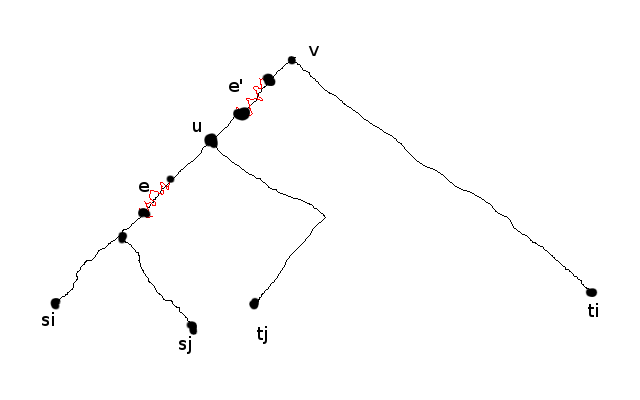
\includegraphics[height=3in]{picture.png}
\end{center}

\subparagraph{Theorem} The algorithm gives a factor-2 approximation.

\textbf{Proof} To show this, we apply approximate primal-dual complementary slackness conditions with $\alpha = 1, \beta = 2$.  Our goal is to show:
\begin{eqnarray*}
\forall e \in E : & d_e \neq 0 \implies & \sum \limits_{i : P_i \ni e} f_i = c(e) \\
\forall 1 \leq i \leq k : &  f_i \neq 0 \implies & \sum \limits_{e \in P_i} d_e \leq 2
\end{eqnarray*}
The first condition is trivially satisfied, since we never over saturate any flow.  For the second condition, the above lemma proves that if there is some flow between $s_i, t_i$, then we never picked more than one cut edge per the path $v$ to $s_i$ and $v$ to $t_i$ (with $v = lca(s_i, t_i)$) and so the total number of cut edges from $s_i$ to $t_i$ is less than 2.  As a result, we obtain a factor $\alpha \beta = 2$ approximation.

\end{document}
